
\chapter{Project Scope}

\begin{figure}[h]
\centering
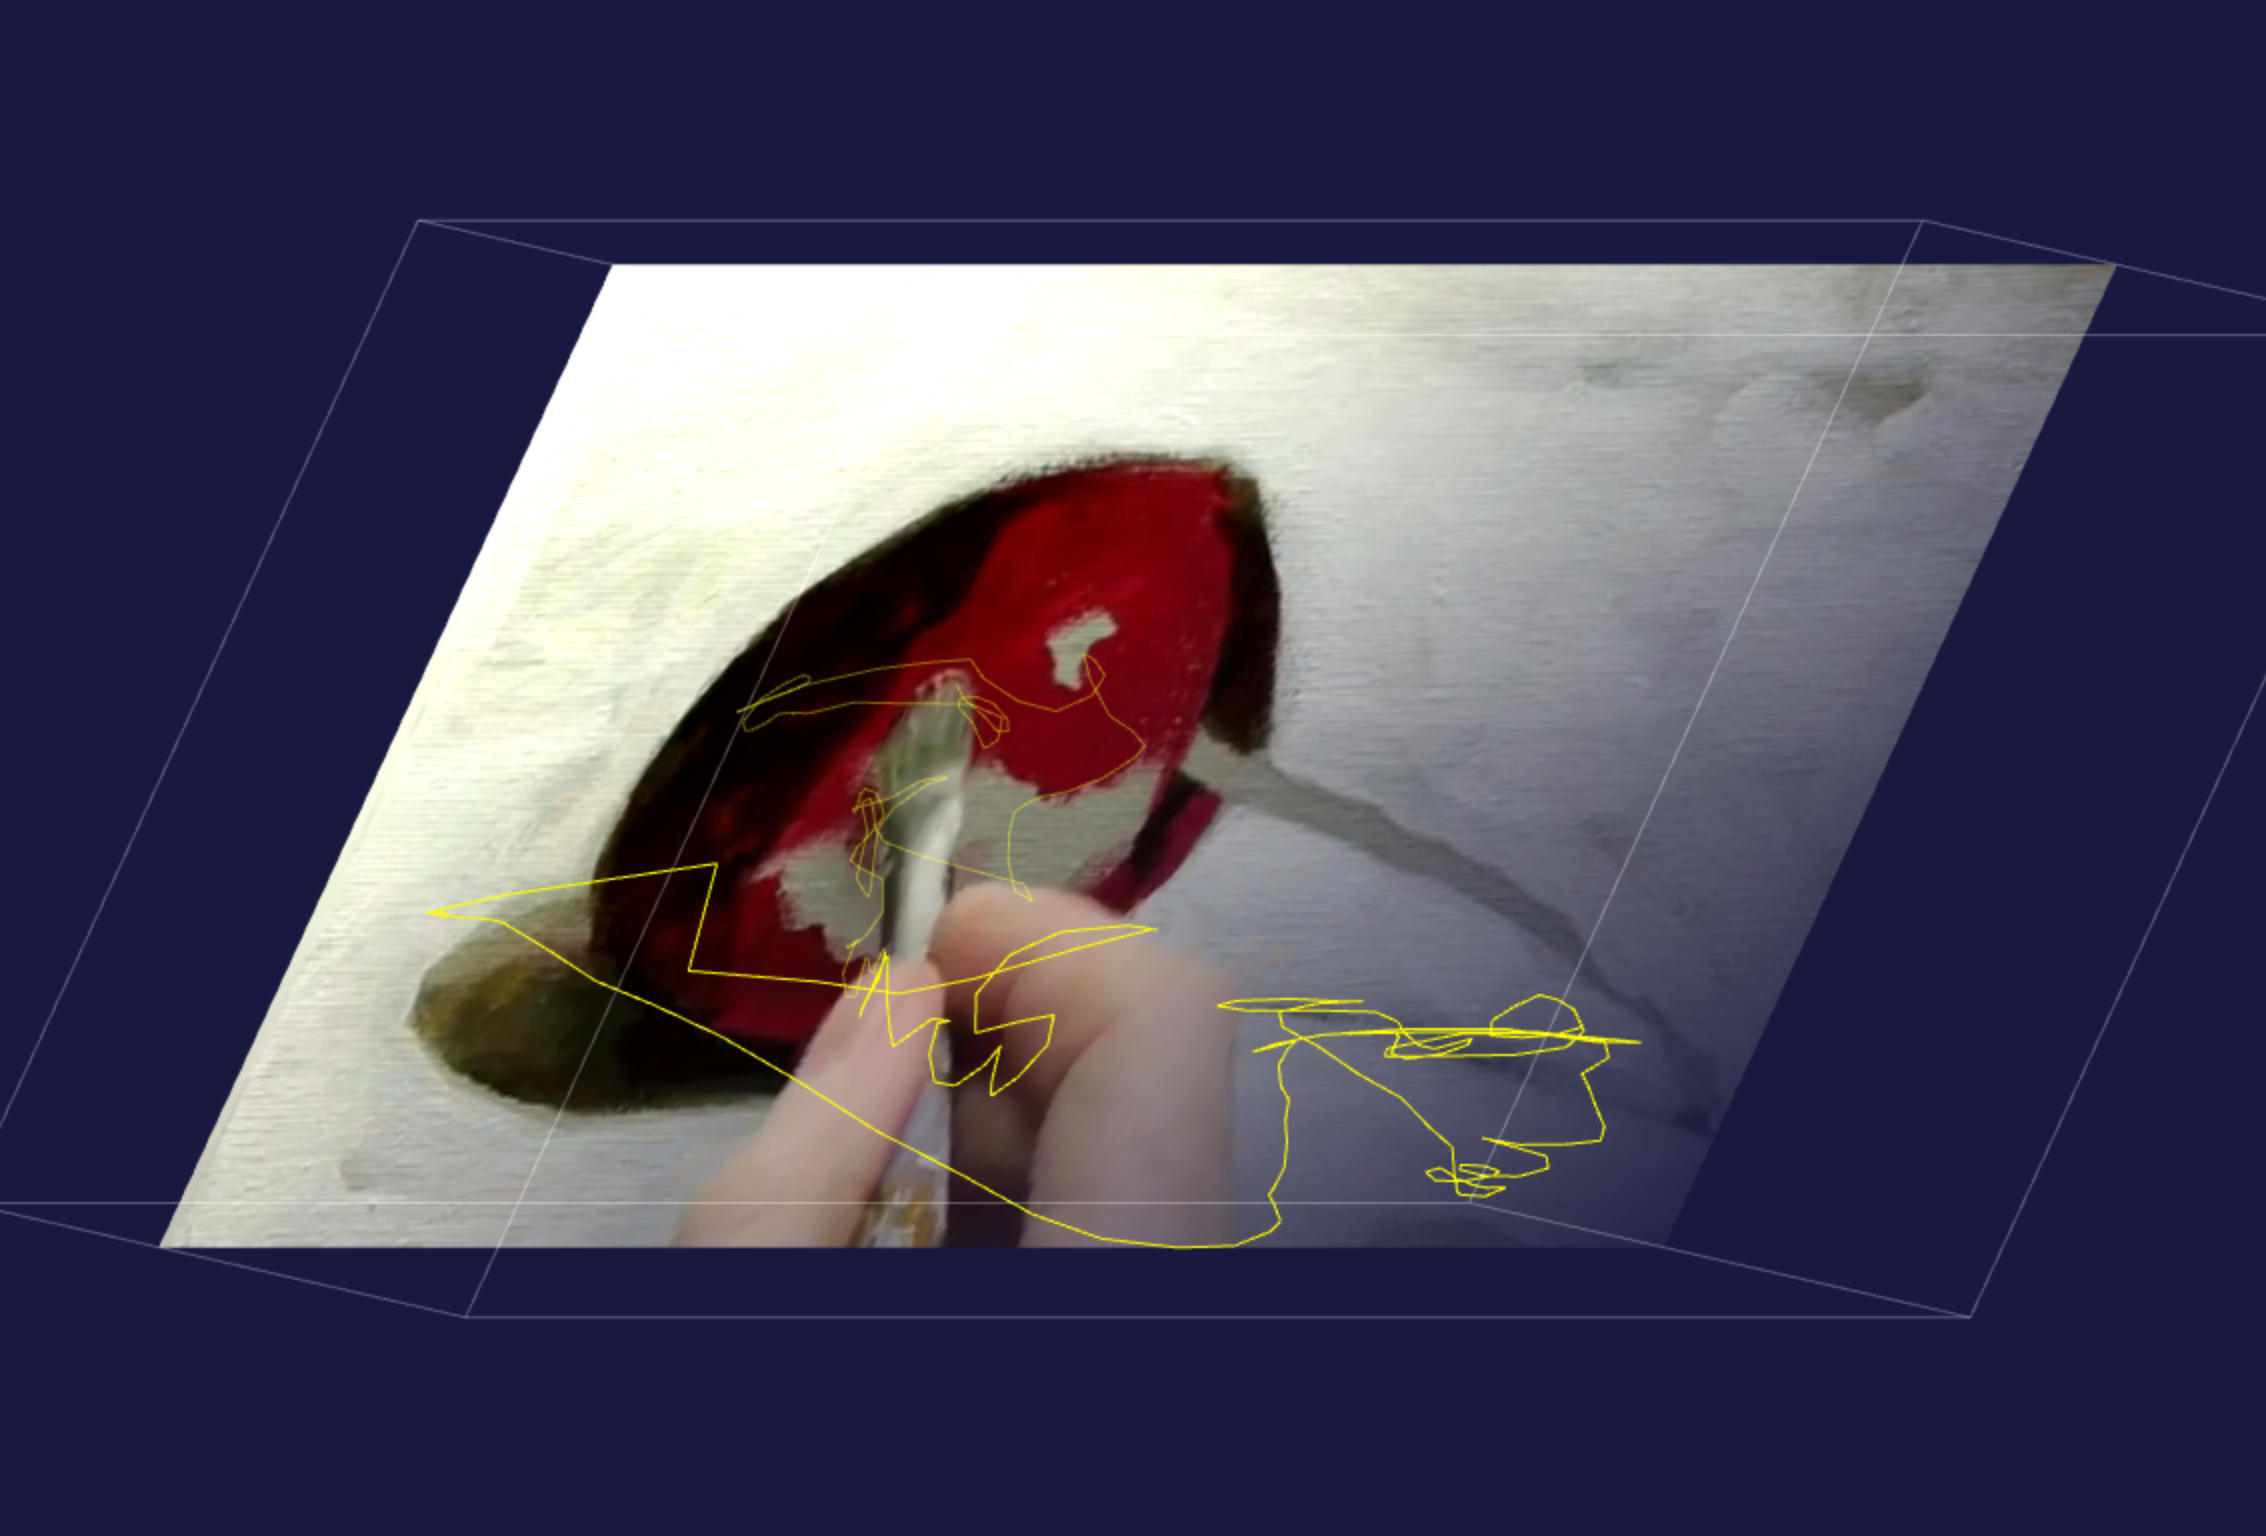
\includegraphics[width=\textwidth]{DMVN}
\caption{Web-based 3D DMVN}
\end{figure}

\section{Goals}

\subsection{Objective}
The objective of this project was to implement a novel method for interactive video navigation, \textbf{\emph{3D Direct Manipulation Video Navigation}} \cite{dmvn3d} (hereforth referred to as \emph{3D DMVN}) as a service remotely accessible via the World Wide Web. The original implementation of 3D DMVN was a native PC executable; porting it to a web-based system requires different considerations in its systems architecture; for example:
\begin{itemize}
    \item a web service is usually accessed through a remote client, and the data transferred from server to client must traverse the World Wide Web;
    \begin{itemize}
        \item server operation cost and expectation of limited client internet bandwidth encourage careful consideration of network usage;
        \item as a consequence, both overall data throughput and transfer latency must be taken into account;
    \end{itemize}
    \item the hardware capabilities of the compute device (PC, phone, tablet, etc) that accesses the service is uncontrollable by the developer;
    \item the client of the service must run in another program, the Web Browser, and operate within its own limitations and security constraints; and
    \item preferably, for the purposes of encouraging widespread adoption as a practical solution, the solution should be built upon a standard Web Server, with no additional, custom back-end services.
\end{itemize}

\subsection{Direct Manipulation Video Navigation}
Direct Manipulation Video Navigation (or \emph{DMVN}) is a proposed method by which a user is enabled to temporally navigate through a video by dragging an \emph{Object of Interest} along a visual representation of its path of motion, instead of through the traditional linear timeline interface. \cite{dmvn}
\par As one example of a DMVN implementation: a user might be able to select an object, be presented with a visualization of its motion trajectory path, and then use the mouse to drag the object through that path of motion, rather than through a timeline.\par
In other words, DMVN allows the user to visualize and interact with a video's seek-time spatially, rather than temporally.

\subsection{\emph{3D} Direction Manipulation Video Navigation}
3D Direct Manipulation Video Navigation (\emph{3D DMVN}) is a proposed extension of DMVN that allows the user to ``rotate" the video and the object path, whose $z$ coordinate corresponds to a unique position in time. This resolves many problems with the original DMVN, including (but not limited to): \cite{dmvn3d}
\begin{enumerate}
\item Temporal Ambiguity;
\item Recurring Motion; and
\item Self-Intersecting Motion.
\end{enumerate}

\subsubsection {Temporal Ambiguity}
    If the object pauses in place for some period of time, then the user will have no way to select any specific point of time in that interval with DMVN, since the path remains a constant $(x,y)$ throughout that entire period of immotion. 3D DMVN resolves this, since \emph{time} is given its own axis on the path $(x,y,t)$, which can easily be seen and selected by the user by rotating the view.
\subsubsection{Recurring Motion}
    If an object's motion trajectory demonstates recurring motion (for example, the pendulum of a clock), the simpler DMVN's motion path would be self-occlude, making the selection of a specific point in time impossible; when a user clicks, should it select the first time the motion recurred? Second? 3D DMVN resolves this again through the temporal axis, which makes redundant points impossible.
\subsubsection{Self-intersecting Motion}
    If the motion trajectory ever crosses itself and a user is dragging along the path, traditional DMVN doesn't provide enough information to resolve which path to continue along to provide a temporally continuity of navigation. Again, 3D DMVN resolves this by ensuring that every point on the path has a unique coordinate, and thereby avoids confusion during the navigation process.
\section{Limitations}
This project is \emph{not} meant to create a production-ready, polished product, but rather to serve as a \emph{proof of concept} of a web implementation of 3D DMVN, and hopefully someday be of use as a foundation for demonstrating that DMVN can be practically useful in everyday applications.
\begin{itemize}
    \item Does not implement the optional \emph{Perspective Correction} described in the 3D DMVN paper, as it would not have been well suited for the example videos, and seemed outside the scope of effort.
    \item Leaves user-interface development for \emph{mobile devices}\cite{fatfinger} for future development, as again this would be extra effort on the client beyond the scope of the client-server architecture as a whole, and could become a distraction from the project's scope.
    \item Emphasizes development for static web servers, as they are commonly accessible. However, discussion and comparison of static vs. dynamic web server approaches \emph{is} included in this report.
\end{itemize}

\section{Materials}
The author of the 3D DMVN paper graciously provided materials from his research for my implementation. These included:
\begin{itemize}
    \item Two example videos in AVI container format, well-suited to illustrate 3D DMVN:
    \begin{itemize}
    \item \textbf{\emph{Gym}}: a scene where a man uses a weight machine. The scene is largely immobile, except for the man's arms and the weight pulley system. Both of these objects under motion repeat their paths in a self-occluding fashion (when viewed in 2D DMVN), and thus provides an example of the utility of 3D DMVN.
    \item \textbf{\emph{Painting}}: a close-up scene where an artist paints with a paintbrush. This scene offers some challenges due to the complicated path of the brush, and the close-up field of view causes parts of the painter's hand and brush to leave the video for periods of time.
    \end{itemize}
    \item Uncompressed binary data files relating to the above two videos.
\end{itemize}

\section{Tools}
I wanted to use the most basic toolset possible, eschewing third-party libraries (as much as practical) in order to keep the majority of the implementation manual, for educational purposes.
\begin{itemize}
\item \textbf{\texttt{vim}} for the authoring of this report and all project code;
\item \textbf{\texttt{python}} language and interpreter,
    \begin{itemize}
    \item along with the popular \verb!numpy! and \verb!opencv! libraries for the purposes of performance;
    \item \verb!python! was chosen because I was unfamiliar with the language (making for a good learning experience), and because it seemed like it would make a good compromise between coding efficiency and runtime performance (when utilizing C-based libraries such as above)
    \end{itemize}
\item \textbf{\texttt{html}}\&\textbf{\texttt{css}} markup languages for the description and styling of the client-side web page;
\item \textbf{\texttt{javascript}} for front-end development, as it remains the only native client-side language for the web, using only:
    \begin{itemize}
    \item the \verb!underscore! functional library for the \verb!_.flatten! function, which reinterprets multidimensional arrays as single-dimensional
    \item the matrix and vector function library \verb!mat.js! was written manually by myself for educational purposes;
    \item it should be noted that I purposefully avoided higher-level 3D libraries, such as \verb!three.js!, since I felt that it would take away from the effort of the project and might compromise the results;
    \end{itemize}
\item Google \textbf{Chrome} browser for viewing and debugging of the web front-end; and
\item \textbf{\LaTeX} for formatting of this report, since I had never used it before and figured now would be as good a time as any to learn.
\end{itemize}

\section {Deliverables}
The following deliverable items are included with this project submission:
\begin{itemize}
    \item \href{http://web.cecs.pdx.edu/~bargerm/dmvn/dmvn.pdf}{\textbf{Project Report}} (this document): \url{http://web.cecs.pdx.edu/~bargerm/dmvn/dmvn.pdf};
    \item \href{http://web.cecs.pdx.edu/~bargerm/dmvn/dmvn.html}{\textbf{Interactive Demonstration Website}}, best used with the Google Chrome browser: \url{http://web.cecs.pdx.edu/~bargerm/dmvn/dmvn.html};
    \item \href{http://web.cecs.pdx.edu/~bargerm/dmvn/res/dmvn.mp4}{\textbf{Demonstration Video}}: \url{http://web.cecs.pdx.edu/~bargerm/dmvn/res/dmvn.mp4}; and
    \item \href{https://github.com/MichaelABarger/Web3DDMVN}{\textbf{Github Repository}} of all relevant source code: \url{https://github.com/MichaelABarger/Web3DDMVN}.
\end{itemize}

